\newpage

\chapter{Framework for Generating Splitting Criteria for Multi-valued Attributes}
\label{chap:framework}

First we recall some definitions and results for the Max-Cut problem. These definitions will be used in the following section, when we define our framework.

\section{The Maximum Weighted Cut Problem}
\label{sec:maxcutbackground}

We  recall some definitions from graph theory. A cut  $X$ in  a weighted graph $G=(V,E)$ is
a subset of vertexes of $V$. The weight of a cut $X$, denoted here by $w(X)$, is the sum of the weights
of the edges that have one endpoint in $X$ and the other one in $V-X$.

The problem of computing the  cut $X^*$ with maximum weight in a graph with non-negative weights is NP-Hard.
However, there are good  approximation algorithms
available. A remarkable one is the randomized algorithm
 proposed in  \cite{GoeWil95} that relies on a formulation of
the max-cut problem via semidefinite programming (SDP). This algorithm,  denoted throughout this dissertation by GW, 
returns a cut $X$ that satisfies  $E[w(X)] \ge 0.878 w(X^*)$. It involves solving an SDP on the graph weights matrix, calculating the Cholesky decomposition of it and then generating a random partition of the values based on the inner product of the decomposition column vectors with a randomly generated vector on the sphere of dimension $n$. As solving such an SDP takes $O(n^4)$ arithmetic operations (see \cite{navascues2009power}) and calculating the Cholesky decomposition takes $O(n^3)$ operations, the time complexity is high but polynomial.

Another possibility to solve the Max-Cut problem is by using the {\tt GreedyCut} algorithm, presented in Algorithm \ref{alg:greedy}. It
obtains a cut $X$ such that $w(X)  \ge 0.5 w(X^*)$, as proved in \cite{SahGon:76}.
The algorithm starts with two empty sets $X$ and $X'$. Then, it
scans the nodes 
and assigns each of them to the set that provides
the maximum improvement on  the weight of the current cut (ties are broken arbitrarily). Is it easy to see that the time complexity of this greedy algorithm is $O(n^2)$.


\begin{algorithm}[tb]
   \caption{ GreedyCut($V$: set of nodes)}
   \label{alg:greedy}
\begin{algorithmic}
\STATE{$X \leftarrow \emptyset$;$X' \leftarrow \emptyset$}
\FOR{$j=1,..,n$ }
\STATE{{\bf If} $$\sum_{v \in X} w(v_i,v) > \sum_{v \in X'-V} w(v_i,v) $$ add $v_i$ to $X'$ {\bf Else} add $v_i$ to $ X$  }
\ENDFOR
\STATE{{\bf Return} $X$ and $X'$ }

\end{algorithmic}
\end{algorithm}


The solutions obtained by both GW and {\tt GreedyCut} 
can be improved via a local search.
In its simplest version, it
moves a node from one group to
the other while some improvement on the cut weight is possible.
Although this algorithm is not polynomial  in the worst case,
it has polynomial behavior in the smoothed analysis framework (see \cite{journals/corr/AngelBPW16}). In addition, it is always possible
to set a limit on the number of moves.
A more refined version  allows exchanging a pair of nodes
as long as the weight of the cut is improved.
In our experiments this is the version we use, as presented in Algorithm \ref{alg:localsearch}.


\begin{algorithm}[tb]
   \caption{ LocalSearch($X$, $X'$): set of nodes}
   \label{alg:localsearch}
\begin{algorithmic}
\STATE{$label:~loop$\_$start$}
\FOR{$i = 1, ..., n$ }
\IF{switching $v_i$'s side improves cut weight}
\STATE switch $v_i$ and update cut weight, $X$, $X'$
\STATE $goto~ loop$\_$start$
\ENDIF
\ENDFOR
\FOR{pair $(v_i, v_j) \in X \times X'$ }
\IF{switching $v_i$ and $v_j$ improves cut weight}
\STATE{switch $v_i$ and $v_j$, update cut weight, $X$, $X'$}
\STATE{$goto~ loop$\_$start$}
\ENDIF
\ENDFOR
\STATE{{\bf Return} $X$, $X'$}

\end{algorithmic}
\end{algorithm}


\section{A Framework for Generating Splitting Criteria}
\label{sec:maxcut}
In this section we explain 
our approach to building binary splitting criteria
for  multi-valued nominal attributes.

Let $A$ be a nominal attribute  that takes
values in the domain $V=\{v_1,\ldots,v_n\}$.
Our framework to produce a splitting criterion $I$ 
consists of three steps:

\begin{enumerate}
\item  Create a complete graph $G=(V,E)$ with $n$ vertexes.

\item  Assign a non-negative weight $w_{ij}$ to the edge 
that connects $v_i$ to $v_j$. This value shall reflect the benefit of putting  $v_i$ and $v_j$ in different partitions.
Different definitions of $w_{ij}$ yield to different criteria,
as we explain further.

\item  Ideally, the value of the criterion $I$ for attribute
$A$ is the weight of the cut with maximum weight  in $G$.
However, this is not a reasonable possibility for large $n$ since, as mentioned before, the problem of computing the  cut $X^*$ with maximum weight in a graph with non-negative weights is NP-Hard.
Thus, the value of criterion $I$ is given by the weight
of the cut obtained by some  algorithm, with approximation guarantee, for the maximum cut
problem in $G$.   
\end{enumerate}

What distinguishes the  criteria
generated  by our framework
is how the weights of the edges are set and what 
method is employed to compute the cut on graph $G$.
Here, we discuss two ways to set the weights:
the first one yields to criteria that
are related with the Gini Gain, while the second 
is built upon some given splitting  criterion that works well for binary attributes.


\subsection{The Squared Gini Criterion}
Here, we discuss how to set the weights so that we obtain 
a criterion that can be seen as a variation of the Gini Gain discussed in Section \ref{def:Gini}.

In fact, Lemma \ref{lem:GiniSq} below  show that  it is possible to define the
weights of the edges so that 
\begin{equation}
 \label{lem:squaredgini}
w(S_L)= Gini(S) - p^2_L \cdot Gini(S_L) - p^2_R \cdot Gini(S_R) 
\end{equation}
for every partition $(L,R)$ of $V$. 

Note that the weight of the cut  $S_L$ in the above identity 
is similar to the expression for the Gini Gain given by equation (\ref{eq:Ginigain}).
The difference is that $p_L$ and $p_R$ are replaced with
$p_L^2$ and $p_R^2$, respectively. Because of the squares, this new criterion tends to favor more balanced partitions. Another practical observation is that one can define the edges without the $2/N^2$ term in \ref{lem:squaredgini} and find the same maximum cut, since this constant appears in all edges weights.

For the proof of Lemma \ref{lem:GiniSq}, recall that $A_{ix}$ is the number
of samples of  class $x$ that have value $v_i$, and that $C$ is used to denote the set of classes.


\begin{lemma}
For every $i,j$, with $i \ne j$ and $i,j \in \{1,\ldots,n\}$,  let
\begin{equation}
 \label{eq:squaredgini}
w_{ij} = \frac{ 2 \sum_{ x,y \in C \atop x \ne y }  A_{ix} A_{jy} }{ N^2} 
\end{equation}
Then, for every partition $(L,R)$ of  $V$ we have
$$w(S_L)=Gini(S) - p^2_L \cdot Gini(S_L) - p^2_R \cdot Gini(S_R)$$
\label{lem:GiniSq}
\end{lemma}

\begin{proof}
Let $S_{x,L}$ and $S_{y,R}$  be the number of samples of classes $x$ and $y$ in groups $L$
and $R$, respectively. Moreover, let  $N_L$ and $N_R$ be 
the number of samples in $L$ and $R$, respectively.
It follows from equation (\ref{eq:gini}) that
$$N^2 Gini(S)=  N^2 -  \sum_{x=1}^k (S_{x,L} + S_{x,R})^2 $$
$$N_L^2 Gini(S_L)=  N_L^2 - \sum_{x=1}^k S_{x,L}^2 $$
and
$$N_R^2 Gini(S_R)= N_R^2 - \sum_{x=1}^k S_{x,L}^2. $$ 
Since $N=(N_L+N_R)$ it follows that 
$$N^2 Gini(S) - N_L^2 Gini(S_L)  - N_R^2 Gini(S_R) =$$
$$ 2 N_L N_R - 2 \sum_{x \in C} S_{x,L} S_{x,R} = $$
$$ 2  \sum_{x \in C } S_{x,L} \sum_{x \in C} S_{x,R}  - 2 \sum_{x \in C} S_{x,L} S_{x,R} =$$  
$$ 2  \sum_{ x \neq y \atop x,y \in C } S_{x,L} S_{y,R} =  2 \sum_{ x \neq y \atop x,y \in C } \left ( \sum_{ i \in L   }\sum_{ j \in R   }  A_{ix}A_{jy} \right ) =$$
$$ N^2 \sum_{i \in L  } \sum_{j \in R  } w_{ij} =  N^2 w(S_L) $$
Dividing the first term and the last term by $N^2$ in the  above expression and, using
 $N_L=p_L \cdot N$ and $N_R=p_R \cdot N$,
we  establish 
the lemma.
\end{proof}


It is worth mentioning that symmetric 
misclassification costs can be easily introduced in this case.
In fact, let $mix(x,y)$  be the cost 	
of  mixing  samples from classes $x$ and $y$.
We can define 
$$ w_{ij} =   \sum_{ x,y \in C \atop x \ne y } mix(x,y)  p_{ix} p_{jy} .$$
This measure favors the separation of the classes
that incur  a large cost in the case they are mixed.

Another natural question is whether the maximum weighted cut problem, which is NP-complete in general, is not easier for the case where the weights are set by equation \ref{eq:squaredgini}. The answer is no, as proved in the theorem below.

\begin{theorem}
Finding the maximum weighted cut in a complete graph whose weights are set by equation \ref{eq:squaredgini} is NP-complete.
\end{theorem}

\begin{proof}
 The idea is to show a reduction from the NP-complete problem PARTITION using the fact that, for some specific instances of our problem, the optimal partition is the most balanced one.
 
 Recall that, in the PARTITION problem, we are given a multiset of integers and want to decide whether it can be partitioned into two multisets with the same sum of elements. Consider an instance given by a multiset $U = \{u_1, \ldots, u_k\}$ of integers. Create an instance of our decision tree problem as follows: for each $u_i \in U$ add a value $v_i$ whose row in the contingency table is given by $u_i e_i$. In other words, in this instance every value has a single class and every class appears for a single value. Hence, every edge $w_{ij}$ in the associated Squared Gini graph will have weight equal to $ij$. Therefore, any cut partitioning $V$ into $(L, R)$ will have value equal to
 $$cut(L, R) = \Big(\sum_{i|v_i \in L} u_i\Big) \cdot \Big(\sum_{i|v_i \in R} u_i\Big)$$
 
Note that this formula is maximized when the two terms are as close as possible, i.e. the two partition sides are as balanced as possible. Thus, if we can find a polynomial time algorithm that finds the best partition of this instance's values, we can solve the associated PARTITION problem. This concludes the reduction.
\end{proof}

\subsection{Setting weights according to other splitting criteria}

Our second way of defining the weights makes use of some 
given splitting criterion 
for  binary nominal attributes. 
Such  criterion is used to measure the quality of separating samples with value $v_i$ from those with value $v_j$,
for each $i$ and $j$, and, thus, defining the edges' weights.
Here, we investigate the criterion obtained by 
defining $w_{ij}$ as the value of the $\chi^2$-test
for the attribute $A$ when  evaluated over the restricted dataset 
that contains only the samples of $S$ with values $v_i$ and $v_j$:
$$w_{ij}=  \sum_{\ell=1}^k \frac{(A_{i \ell}-E[A_{i \ell}] )^2}{E[A_{ i \ell}]}
+ \sum_{\ell=1}^k \frac{(A_{j \ell}-E[A_{j \ell}] )^2}{E[A_{ j \ell}]}
$$
where $E[A_{i \ell }]=N_i p_{\ell}$
and $E[A_{j \ell }]=N_j p_{\ell} $.

In order to reduce the bias towards attributes with many values, we divide 
$w_{ij}$ by  $n-1$, for every pair $(i,j)$. We make this adjustment  because each value contributes
to the weight of $n-1$ edges.

We shall remark that, although not explored in this work,
other criteria such as Information Gain or Gini Index
could be used, instead of the $\chi^2$-test, to
set the weights.


\subsection{Example}

Let's assume the are using the Squared Gini criterion on a dataset with a single attribute (the marital status) and we try to predict whether it's a male or female. The contingency table and associated Squared Gini graph are given in figure \ref{fig:cut-example}.

Since this example is small (there are only $7$ non-empty distinct cuts), we can run through all the possible cuts and see that the one shown in red is actually the maximum one. In larger examples we need to use approximated algorithms such as the one mentioned before, since the number of possible cuts grows exponentially with the number of nodes/values.

\begin{figure}[h]
\centering
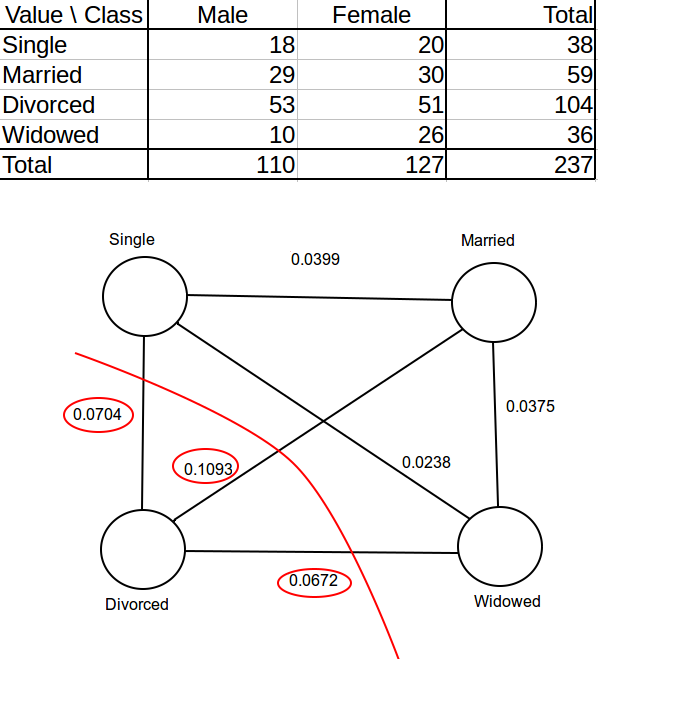
\includegraphics[width=0.75\textwidth]{cut-example2}
\caption{Contingency table, associated Squared Gini graph and maximum cut.}
\label{fig:cut-example}
\end{figure}

\subsection{Handling Numeric Attributes}
We observe  that criteria from our framework can handle
 a numeric attribute $A$ with $t$ distinct values
$v_1,\ldots,v_t$
by considering it as collection of 
$t-1$ binary attributes, where the
$j$-th attribute, $A^j$,  splits the samples into the
groups $\{s | A(s) \le v_j \}$ and $\{s | A(s) > v_j \}$. 
The split  obtained by criterion $I$ on a numeric attribute
$A$ matches the split of  the best attribute 
among $A^1,\ldots,A^ {t-1}$, according to $I$.
